\chapter{基于BLE Mesh的智能家居平台功能设计}

\section{架构设计}
本项目主要分为三个部分:BLE Mesh节点,网关端及移动端,如图~\ref{fig:arch}。

BLE Mesh节点主要实现传感器、继电器、灯泡等设备的接入,并且节点间可自动建立BLE协议下的Mesh网络,使得用户即使不使用网关也能用移动端软件连接至Mesh网络控制所有节点。

网关端主要实现设备层与管理应用层的连接。采用插件化的方案,使得有能力的爱好者或其他智能设备厂商,可以自己根据本项目简单的API来制作插件接入本平台;也便于接入到其他的管理平台,例如Apple HomeKit、Google Home等,让用户不需要下载其他程序就能管理网关下的所有设备。

移动端主要实现控制Mesh网络或网关下的设备、添加自动化的功能。
\begin{figure}[H]
    \centering
    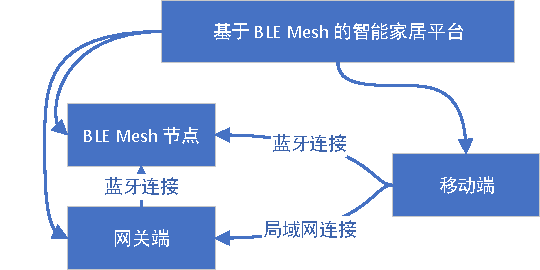
\includegraphics{arch_basic.pdf}
    \caption{基于BLE Mesh的智能家居平台基本架构图}
    \label{fig:arch}
\end{figure}

\section{BLE Mesh节点}
BLE Mesh节点不同于一般智能家居设备,它们之间通过另一个BLE Mesh分发节点或手机分发配置后构成网状网络,之后所有数据就可通过其他节点转发至目标设备。

每个节点均可接入多个模块,例如继电器、开关、传感器等。不需要每个模块都单独配一套蓝牙通讯装置,节约了成本也节约了频段资源。

网关或移动端设备也可以通过任一节点代理入Mesh网络,之后便可以访问所有的节点及其连接的模块。
\begin{figure}[H]
    \centering
    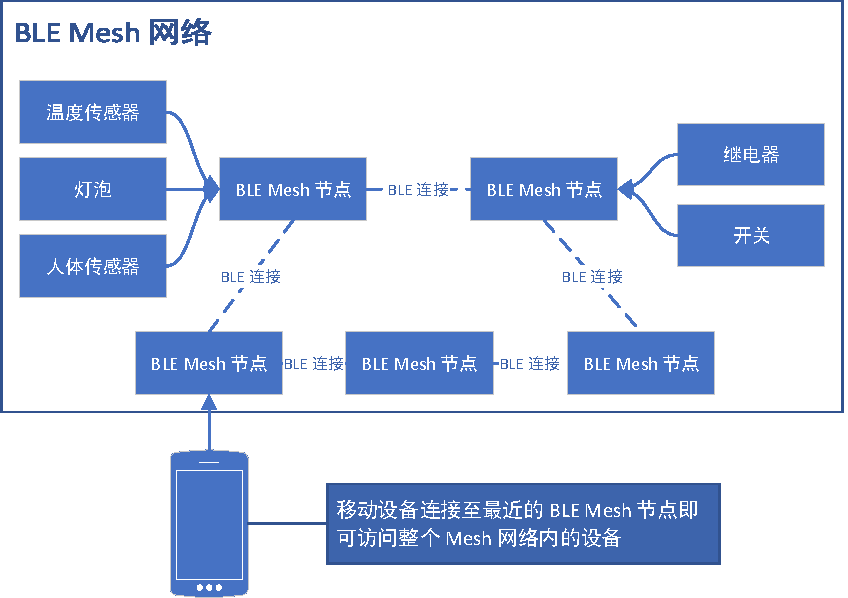
\includegraphics{arch_mesh.pdf}
    \caption{BLE Mesh网络架构图}
    \label{fig:arch}
\end{figure}
\section{网关端}


\section{移动端}
内容
